\documentclass[journal]{IEEEtran}
% Draft v0 (2026-10-17). Numbers in tables are generated by gen_tables.py from the frozen result files;
% numbers in the text are copied from those tables / EXPERIMENT_LOG.md. \todo{} marks open items.
\usepackage{amsmath,amssymb}
\usepackage{graphicx}
\usepackage{booktabs}
\usepackage{multirow}
\usepackage{xcolor}
\usepackage{cite}
\usepackage[hidelinks]{hyperref}
\usepackage[capitalise,nameinlink]{cleveref}
\newcommand{\todo}[1]{\textcolor{red}{[TODO: #1]}}
\newcommand{\R}{\mathbb{R}}

\begin{document}

\title{Bounding the Tail: Multi-Hypothesis Fusion of Cross-View Retrieval and Inertial Motion for GNSS-Free UAV Localization}

\author{\todo{Authors}%
\thanks{\todo{Affiliations, funding.}}}

\maketitle

\begin{abstract}
Cross-view retrieval localizes a UAV by matching its nadir image against geo-referenced satellite tiles, but single-frame
retrieval fails in a heavy-tailed way: on real flights a model trained on another dataset places 5\,\% of the frames
more than 3.7\,km away, and its similarity scores barely predict these failures \todo{support with the GeoAUROC analysis or drop this clause}. We argue that the useful question is
not the mean error but how often, and for how long, a navigation filter is dragged away by such failures. We propose a
multi-hypothesis extended Kalman filter (MH-EKF) that treats the Top-$K$ retrieval candidates as a mixture measurement
with an explicit outlier component, keeps a small bank of Gaussian hypotheses propagated with VIO or a consumer IMU,
gates every candidate against each hypothesis, and restricts re-acquisition to the propagated $3\sigma$ region. We
evaluate on two settings with strict validation/test separation: semi-simulated flights over the real DenseUAV tile
grid, and eight real flights (3.6--9.9\,km) of the AerialVL dataset with simulated inertial data, against motion-only
navigation, a $\chi^2$-gated EKF, a Top-$K$ particle filter and a re-implementation of NaviLoc. With VIO, MH-EKF halves
the p95 error of VIO alone on 10--22-minute flights (95\,$\rightarrow$\,49\,m). Its main benefit is robustness: with a
300\,m start error its p95 is 102\,m versus 404--1168\,m for the other filters, and with an IMU only it is the only
method that does not drift by kilometres. Paired bootstrap tests over flights find MH-EKF significantly better in 187
of 228 comparisons and significantly worse in one (by 2\,m). We also report where it does not help: with VIO and a
correct start, all filters are within a few metres.
\end{abstract}

\begin{IEEEkeywords}
UAV localization, GNSS-denied navigation, cross-view geo-localization, visual place recognition, multi-hypothesis tracking.
\end{IEEEkeywords}

% =====================================================================================================
\section{Introduction}
\IEEEPARstart{G}{NSS} outages and spoofing make absolute visual localization against satellite imagery an attractive
complement to visual-inertial odometry (VIO) for UAVs~\cite{qin2018vins,mourikis2007msckf}. Cross-view geo-localization
models trained on drone--satellite pairs~\cite{zheng2020university,wang2022lpn,dai2022fsra,dai2024denseuav} reach
80--85\,\% Recall@1 on their own benchmark, which suggests that an image-retrieval fix every second could keep VIO drift
bounded.

Two properties of retrieval make this less straightforward than the Recall@1 numbers suggest. First, failures are not
small: a wrong top-1 is usually a visually similar tile far away---another field with the same crop pattern, another
campus with the same building layout. On the real AerialVL flights~\cite{he2024aerialvl}, the 95th percentile of the
single-frame top-1 error is 3.7--3.8\,km for models trained on DenseUAV (\cref{tab:aerialvl}), and fine-tuning on other
flights of the same area reduces the median error to about 30--45\,m but not this tail. Second, failures are
temporally correlated: aliasing persists for tens of seconds along a flight, so a filter that accepts a wrong fix once
is often offered a consistent chain of wrong fixes afterwards. A filter tuned for Gaussian measurement noise is
therefore either too trusting (and is hijacked) or too strict (and rejects correct fixes after its own error has grown).

Recent systems fuse retrieval or map matching with odometry~\cite{he2023foundloc,shpagin2026naviloc,li2025geovins,swapf2025},
and report mean or trajectory errors. We focus instead on the \emph{tail}: the p95 error and the fraction of time a
filter is lost (more than 100\,m off), across conditions that stress the filter rather than the retrieval model: an
IMU-only motion source, a wrong start position, and long flights.

\textbf{Contributions.}
\begin{itemize}
  \item A multi-hypothesis EKF over the Top-$K$ retrieval candidates with an explicit outlier component, per-hypothesis
  $\chi^2$ gating and covariance-bounded re-acquisition, for both VIO and raw-IMU motion models (\cref{sec:method}).
  \item An evaluation protocol centred on tail metrics with flight-level paired bootstrap confidence intervals, and with
  every design choice made on validation flights or campuses before a single test run (\cref{sec:setup}).
  \item Experiments on semi-simulated DenseUAV flights and on eight real AerialVL test flights, against motion-only
  navigation, a gated EKF, a Top-$K$ particle filter and a re-implementation of NaviLoc~\cite{shpagin2026naviloc},
  including an ablation and an honest account of the regimes where the method brings no gain (\cref{sec:results}).
\end{itemize}

% =====================================================================================================
\section{Related Work}
\textbf{Cross-view geo-localization and VPR.} University-1652~\cite{zheng2020university} established drone-to-satellite
retrieval; LPN~\cite{wang2022lpn} and FSRA~\cite{dai2022fsra} add part-based pooling and region alignment;
DenseUAV~\cite{dai2024denseuav} densifies the satellite gallery to evaluate positioning error rather than class
identity. General-purpose VPR descriptors~\cite{arandjelovic2016netvlad,keetha2023anyloc} transfer across domains but
are weaker on the nadir aerial-to-satellite gap. These works evaluate single images; we use their Top-$K$ output as a
noisy measurement.

\textbf{Fusing absolute visual fixes with odometry.} FoundLoc~\cite{he2023foundloc} combines VIO with foundation-model
VPR. NaviLoc~\cite{shpagin2026naviloc} aligns a VIO trajectory to top-1 retrieval targets with a robust (median-based)
SE(2) estimate followed by sliding-window refinement; it is training-free and batch. GeoVINS~\cite{li2025geovins}
tightly couples VIO with geographic map registration on AerialVL. SWA-PF~\cite{swapf2025} runs a particle filter
against a semantic map instead of retrieval. These methods report mean or trajectory errors on a few flights; tail
behaviour and the IMU-only case are rarely analysed.

\textbf{Multi-hypothesis estimation.} Gaussian-sum filters~\cite{alspach1972gaussiansum} and multiple-hypothesis
tracking~\cite{reid1979mht} represent multimodal posteriors with a bank of Kalman filters; Monte Carlo
localization~\cite{dellaert1999mcl} and MHT-based global localization~\cite{jensfelt2001mht} address the kidnapped-robot
problem. Our filter is a pragmatic instance of this family whose hypotheses are spawned from retrieval candidates and
whose re-acquisition is restricted to avoid jumping to aliases.

% =====================================================================================================
\section{Method}\label{sec:method}
\subsection{Problem and measurements}
The UAV flies at roughly constant altitude over a geo-referenced satellite map cut into overlapping square tiles with
known centres $\{\mathbf{g}_j\}$. At each tick $t$ (1\,Hz) a retrieval model returns the $K$ most similar tiles
$\mathcal{C}_t=\{(\mathbf{c}_{t,k}, s_{t,k})\}_{k=1}^{K}$ (tile centre, cosine similarity). Between ticks, a motion
source provides either VIO body velocities (10\,Hz) or raw accelerometer and gyroscope readings (100\,Hz). We estimate
the horizontal position $\mathbf{p}_t\in\R^2$; heading is known up to the VIO yaw error or estimated by the INS.

\subsection{Motion models}
\emph{VIO.} The state $\mathbf{x}=[\mathbf{p}, \delta\psi, s, \mathbf{b}]$ holds position, a slowly varying yaw offset
of the VIO frame, a scale error and a velocity bias. The VIO velocity $\mathbf{u}$ is mapped to the world frame as
$\dot{\mathbf{p}} = R(-\delta\psi)\,(\mathbf{u}-\mathbf{b})/(1+s)$, with random-walk models for $\delta\psi$ and $\mathbf{b}$.
\emph{IMU.} An 8-state planar strapdown INS $[\mathbf{p},\mathbf{v},\psi,\mathbf{b}_a, b_g]$ integrates the
accelerometer (rotated by $\psi$, minus bias) and gyroscope. Both are standard EKF prediction steps.

\subsection{Mixture measurement model}
Each candidate is a possible position fix with isotropic noise $\sigma_m$ (one tile step), and the whole retrieval may be
wrong with probability $\varepsilon$. With softmax weights $\pi_{t,k}\propto\exp(s_{t,k}/\tau)$,
\begin{equation}
p(\mathcal{C}_t\mid\mathbf{p}) = (1-\varepsilon)\sum_{k}\pi_{t,k}\,\mathcal{N}(\mathbf{c}_{t,k};\mathbf{p},\sigma_m^2 I)
+ \varepsilon\,\frac{1}{A},
\label{eq:mix}
\end{equation}
where $A$ is the area of the uniform outlier density.

\subsection{Multi-hypothesis update}
The posterior is a weighted bank $\{(w_i,\hat{\mathbf{x}}_i,P_i)\}_{i\le M}$. At each measurement every hypothesis $i$
branches into (a) an \emph{outlier} child that keeps $(\hat{\mathbf{x}}_i,P_i)$ with weight $w_i\varepsilon/A$, and
(b) one child per candidate $k$ that passes the gate
$d^2_{ik}=\boldsymbol{\nu}_{ik}^\top S_i^{-1}\boldsymbol{\nu}_{ik}<\chi^2_{2,0.99}$, with
$\boldsymbol{\nu}_{ik}=\mathbf{c}_{t,k}-\hat{\mathbf{p}}_i$ and $S_i=P_i^{pp}+\sigma_m^2I$. A candidate child receives a
standard EKF update and the weight $w_i(1-\varepsilon)\pi_{t,k}\,\mathcal{N}(\boldsymbol{\nu}_{ik};\mathbf{0},S_i)$.
Children closer than $d_{\mathrm{merge}}$ are merged (weights summed, the heavier child kept) and the $M$ heaviest are
retained. The output is the mean of the heaviest hypothesis.

\subsection{Loss detection and bounded re-acquisition}
The track is declared \emph{unsupported} when no candidate falls inside the gate of the heaviest hypothesis. After
$n_{\mathrm{reacq}}$ consecutive unsupported measurements, new hypotheses are spawned on the current candidates, but
only on those within $3\sigma$ of the heaviest hypothesis, where $\sigma$ is the largest standard deviation of its
propagated position covariance. Earlier variants that re-acquired anywhere, or within $3\sigma+v_{\max}\Delta t$, were
hijacked by long-lasting aliases on validation flights (\cref{sec:ablation}).

\subsection{Parameters}
All parameters were fixed on validation data: $K=10$, $M=10$, $\sigma_m=20$\,m, $\tau=0.02$, $\varepsilon=0.3$,
$A=10^6$\,m$^2$, $d_{\mathrm{merge}}=15$\,m, $n_{\mathrm{reacq}}=20$, spawn prior $0.05$. The design was frozen before the
test runs and is identical in every table.

% =====================================================================================================
\section{Experimental Setup}\label{sec:setup}
\subsection{Retrieval models}
We re-trained three DenseUAV~\cite{dai2024denseuav} models with a ViT-S backbone~\cite{dosovitskiy2021vit}---single
branch, LPN~\cite{wang2022lpn} and FSRA~\cite{dai2022fsra} heads---with the original code and configuration, each with
three seeds. Their DenseUAV Recall@1 is given in \cref{tab:retrieval}; every fusion result is averaged over the nine
models.

\subsection{DenseUAV, semi-simulated flights}
DenseUAV provides drone images at three altitudes for a dense grid of satellite tiles over 14 campuses, with GPS per
tile. We generate 300-s trajectories (4--8\,m/s, random turns) over the tile grid of the test campuses; at each tick the
measurement is the real Top-$K$ of a real drone image of the tile under the UAV. Two of the four test campuses are used
for validation (design choices), the other two for test only. Each of the 27 cells (3 heads $\times$ 3 retrieval seeds
$\times$ 3 trajectory seeds) contains 100 flights.

\subsection{AerialVL, real flights}
AerialVL~\cite{he2024aerialvl} contains eleven flights over a rural and suburban area with 2-Hz images, GNSS (1.5\,m RMS)
and a geo-referenced satellite map (0.96\,m/px). Images are orientation-fixed; a 200-m centre crop is matched against
28\,340 tiles of 200\,m on a 25-m grid. The three flights of 2023-03-11 and 2023-03-16 are validation flights; the eight
flights of 2023-03-18 (3.6--9.9\,km, 8--22\,min) are test flights and were used once. A constant camera-to-tile offset
(2.5\,m E, 23.4\,m S) is measured on validation flights and removed. A run is a 240-s window (start every 20\,s on
\texttt{short\_trajtr} and 60\,s on \texttt{long\_trajtr} flights) with several inertial noise seeds.

\subsection{Retrieval fine-tuning}\label{sec:ft}
To study the effect of retrieval quality we also fine-tune each model on the two 2023-03-16 flights (1\,823 frames)
with a symmetric InfoNCE loss~\cite{oord2018infonce} between a frame and the map tile at its GNSS position, with in-batch
and random-tile negatives; the learning rate and epoch are selected on the 2023-03-11 flight. The fine-tuned models see
the same map area as the test flights (on other days); they do not demonstrate generalization to unseen areas.

\subsection{Inertial data}
Both datasets lack usable inertial data in their public form, so we simulate it from the ground-truth trajectory (a
smoothing spline through GNSS for AerialVL). VIO: 10\,Hz velocities with 0.1\,m/s noise, 2\,\% scale error, 3$^\circ$
initial yaw error, 0.5$^\circ/\sqrt{\text{min}}$ yaw random walk and a 0.003\,m/s/$\sqrt{\text{s}}$ velocity-bias random
walk ($\approx$1\,\% drift of distance travelled). IMU (consumer grade): 100\,Hz, accelerometer noise 0.05\,m/s$^2$,
bias 0.05\,m/s$^2$, gyroscope noise 0.005\,rad/s, bias 0.003\,rad/s, with bias random walks.

\subsection{Scenarios, baselines and metrics}
Four scenarios: VIO or IMU, each with a known start ($\sigma=10$\,m) or a wrong start ($\epsilon_0$: $\sigma=300$\,m).
Baselines use the same measurements and motion data: \emph{motion only}; \emph{retrieval top-1}; an \emph{EKF} that
takes the top-1 candidate with a $\chi^2$ gate and covariance inflation after repeated rejections; a \emph{particle
filter} (2\,000 particles) with the mixture likelihood~\eqref{eq:mix}; and \emph{NaviLoc}~\cite{shpagin2026naviloc},
re-implemented from its published algorithm (no code is available). For NaviLoc we skip the heading-rectification stage
because the query features are shared by all methods and AerialVL images are already orientation-fixed; we report the
batch version (it uses future frames of the window) with the global rotation limited to $\pm0.2$\,rad, its best variant
on validation data, with its default window ($W=30$, $O=15$, $K=3$), which was also the best on validation.
Metrics: p95 of the per-second position error over all runs, and the percentage of runs that exceed 100\,m at any time
after the initial convergence (60\,s on AerialVL, 30\,s on DenseUAV), called \emph{lost}. Differences are tested with a
paired bootstrap that resamples whole flights (AerialVL) or trajectories (DenseUAV), pooling the three retrieval seeds.

% =====================================================================================================
\section{Results}\label{sec:results}
\begin{table}[t]
\centering
\caption{Retrieval. DenseUAV: Recall@1 (\%) of our re-trained models (mean $\pm$ std over 3 seeds). AerialVL: \% frames whose top-1 tile is within 50\,m of GNSS, zero-shot $\rightarrow$ fine-tuned (val = 2023-03-11 flight; test = 2023-03-18 flights).}
\label{tab:retrieval}
\setlength{\tabcolsep}{3pt}
\small
\begin{tabular}{lcccc}
\toprule
 & DenseUAV & \multicolumn{3}{c}{AerialVL top-1 $\le$ 50\,m} \\
\cmidrule(lr){3-5}
Head & R@1 & val & test short & test long \\
\midrule
ViT-S, single branch & 80.1$\pm$0.4 & 21$\rightarrow$31 & 37$\rightarrow$72 & 28$\rightarrow$53 \\
ViT-S + LPN & 85.0$\pm$1.2 & 23$\rightarrow$32 & 39$\rightarrow$73 & 29$\rightarrow$60 \\
ViT-S + FSRA & 80.9$\pm$0.9 & 21$\rightarrow$30 & 36$\rightarrow$68 & 27$\rightarrow$54 \\
\bottomrule
\end{tabular}
\end{table}

\begin{table}[t]
\centering
\caption{DenseUAV test campuses (semi-simulated flights over the real tile grid, real retrieval Top-$K$). p95 error in metres (\% runs lost after 30\,s); mean over 3 heads $\times$ 3 retrieval seeds $\times$ 3 trajectory seeds (27 cells of 100 flights of 300\,s).}
\label{tab:dense}
\setlength{\tabcolsep}{3.5pt}
\small
\begin{tabular}{lcccc}
\toprule
Method & VIO & IMU & VIO+$\epsilon_0$ & IMU+$\epsilon_0$ \\
\midrule
Retrieval top-1 & 501 (99) & 501 (99) & 501 (99) & 501 (99) \\
EKF, $\chi^2$-gated & 7.2 (0) & 13 (0.3) & 104 (3) & 63 (3) \\
PF, Top-$K$ & 6.5 (0) & 28 (5) & 14 (0.1) & 584 (56) \\
NaviLoc$^\dagger$ \cite{shpagin2026naviloc} & 11 (0) & 263 (88) & 11 (0) & 263 (88) \\
\textbf{MH-EKF (ours)} & \textbf{6.4} (0) & \textbf{11} (0.2) & \textbf{6.5} (0) & \textbf{12} (0.1) \\
\bottomrule
\end{tabular}
\end{table}

\begin{table*}[t]
\centering
\caption{AerialVL test flights (2023-03-18, never used for any design choice). p95 position error in metres, in brackets the percentage of 240-s windows that exceed 100\,m after the first 60\,s (lost). Mean over 3 retrieval heads $\times$ 3 training seeds. $\epsilon_0$: start position error $\sigma=300$\,m. IMU/VIO are simulated from the GNSS trajectory (Sec.~\ref{sec:setup}). Bold: lowest p95 among the filters. $^\dagger$Our re-implementation.}
\label{tab:aerialvl}
\setlength{\tabcolsep}{4pt}
\small
\begin{tabular}{lcccccccc}
\toprule
 & \multicolumn{4}{c}{3 \texttt{short\_trajtr} flights (3.6--4.5\,km)} & \multicolumn{4}{c}{5 \texttt{long\_trajtr} flights (4.4--9.9\,km)} \\
\cmidrule(lr){2-5}\cmidrule(lr){6-9}
Method & VIO & IMU & VIO+$\epsilon_0$ & IMU+$\epsilon_0$ & VIO & IMU & VIO+$\epsilon_0$ & IMU+$\epsilon_0$ \\
\midrule
\multicolumn{9}{l}{\emph{Retrieval fine-tuned on non-test flights (Sec.~\ref{sec:ft})}} \\
Motion only & 106 (20) & 1842 (100) & 753 (97) & 1923 (100) & 95 (17) & 1734 (100) & 759 (97) & 1881 (100) \\
Retrieval top-1 & 2244 (95) & 2244 (95) & 2244 (95) & 2244 (95) & 3261 (100) & 3261 (100) & 3261 (100) & 3261 (100) \\
EKF, $\chi^2$-gated & 41 (7) & 85 (21) & 408 (13) & 430 (25) & 55 (11) & 348 (42) & 1168 (29) & 1532 (52) \\
PF, Top-$K$ & \textbf{36} (0.2) & 583 (54) & 104 (4) & 1926 (93) & 50 (2) & 768 (67) & 603 (16) & 1949 (92) \\
NaviLoc$^\dagger$ \cite{shpagin2026naviloc} & 38 (0) & 1105 (98) & \textbf{38} (0) & 1105 (98) & 404 (9) & 1244 (99) & 404 (9) & 1244 (99) \\
\textbf{MH-EKF (ours)} & 37 ($<$0.1) & \textbf{51} (10) & 40 (2) & \textbf{63} (12) & \textbf{49} (2) & \textbf{195} (31) & \textbf{102} (5) & \textbf{550} (33) \\
\midrule
\multicolumn{9}{l}{\emph{Retrieval zero-shot (trained on DenseUAV only)}} \\
Motion only & 106 (20) & 1842 (100) & 753 (97) & 1923 (100) & 95 (17) & 1734 (100) & 759 (97) & 1881 (100) \\
Retrieval top-1 & 3834 (100) & 3834 (100) & 3834 (100) & 3834 (100) & 3753 (100) & 3753 (100) & 3753 (100) & 3753 (100) \\
EKF, $\chi^2$-gated & 70 (19) & 417 (44) & 1104 (40) & 1758 (57) & 107 (32) & 1234 (71) & 1382 (64) & 2372 (82) \\
PF, Top-$K$ & 39 (0.1) & 641 (61) & 598 (16) & 2080 (94) & 53 (5) & 1022 (76) & 861 (38) & 2162 (97) \\
NaviLoc$^\dagger$ \cite{shpagin2026naviloc} & 402 (24) & 1274 (99) & 402 (24) & 1274 (99) & 1709 (39) & 1871 (100) & 1709 (39) & 1871 (100) \\
\textbf{MH-EKF (ours)} & \textbf{38} (0) & \textbf{64} (18) & \textbf{148} (4) & \textbf{321} (21) & \textbf{50} (4) & \textbf{463} (48) & \textbf{612} (18) & \textbf{1154} (53) \\
\bottomrule
\end{tabular}
\end{table*}


\subsection{Retrieval}
\Cref{tab:retrieval} shows the gap the filter must bridge. Zero-shot, 27--39\,\% of the AerialVL test frames have a
top-1 within 50\,m; fine-tuning on two other flights roughly doubles this (e.g., LPN: 29\,$\rightarrow$\,60\,\% on the
long flights), but the p95 top-1 error stays above 2\,km (\cref{tab:aerialvl}).

\subsection{DenseUAV}
On the semi-simulated flights (\cref{tab:dense}) MH-EKF has the lowest p95 in all four scenarios and loses at most
0.2\,\% of the flights. The gated EKF is competitive with a known start but loses 3\,\% of the flights with a wrong
start; the particle filter fails with an IMU only (56\,\% lost with a wrong start), as its particles lose diversity in
velocity and bias after resampling. NaviLoc is reasonable with VIO (11\,m) but cannot correct IMU drift, since it only
fits a rigid SE(2) transform to the motion track.

\subsection{AerialVL real flights}
\Cref{tab:aerialvl} and \cref{fig:cdf,fig:lost} summarize the real flights.
\emph{With VIO and a known start}, every filter is within a few metres (fine-tuned retrieval, long flights: MH-EKF 49\,m,
PF 50\,m, EKF 55\,m) and halves the p95 of VIO alone (95\,m). This is the regime where our method brings no gain over a
particle filter.
\emph{With a wrong start}, MH-EKF converges in most windows (\cref{fig:lost}, top) and reaches a p95 of 102\,m versus
603\,m (PF), 404\,m (NaviLoc) and 1\,168\,m (EKF) on the long flights.
\emph{With an IMU only}, the EKF, the PF and NaviLoc follow the inertial drift in many windows, while MH-EKF stays
anchored (p95 195\,m, 31\,\% lost after 60\,s, versus 348--1\,244\,m and 42--99\,\%). This scenario is still not
solved: about a third of the long-flight windows are lost.
Better retrieval helps every filter, and MH-EKF the most in the hard scenarios: with a wrong start on the long flights
its p95 drops from 612\,m (zero-shot) to 102\,m (fine-tuned).

\textbf{Statistical significance.} Over the 228 paired comparisons (four data configurations of AerialVL and DenseUAV,
3 heads, 4 scenarios, 4 competitors), MH-EKF has a significantly lower p95 in 187 and a significantly higher p95 in one
(fine-tuned retrieval, short flights, LPN, wrong start: +2\,m [+1, +2] versus NaviLoc). The non-significant cases are
mainly the PF with VIO (differences of 0--1\,m) and NaviLoc on the long flights, where five flights give wide intervals.

\begin{figure*}[t]
  \centering
  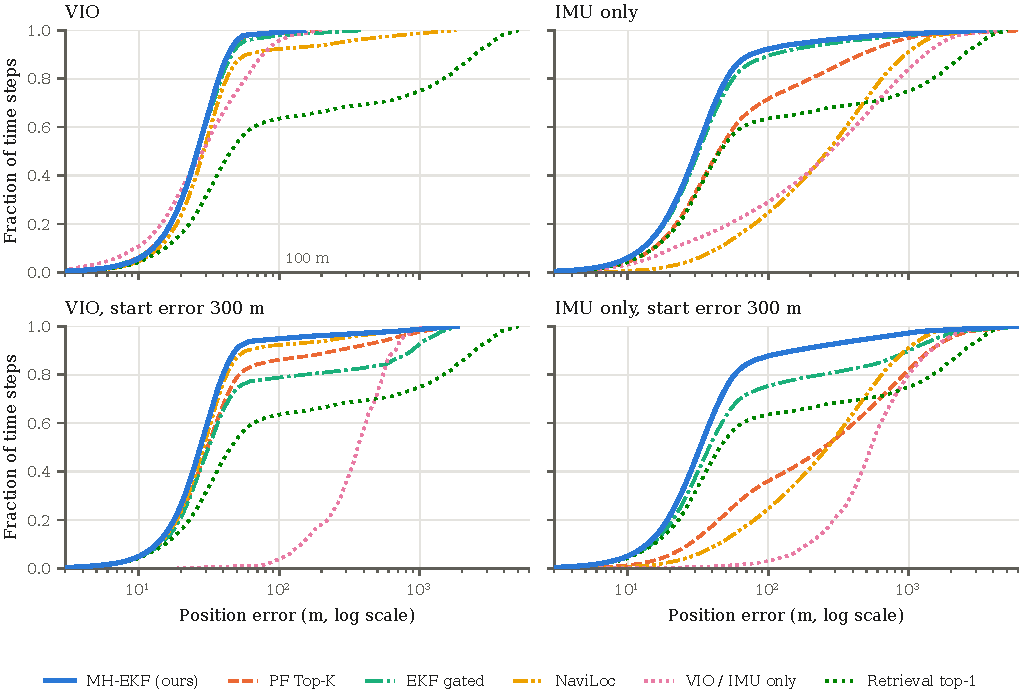
\includegraphics[width=0.92\textwidth]{figs/fig_cdf_long_ft.pdf}
  \caption{Error CDF on the five AerialVL \texttt{long\_trajtr} test flights (fine-tuned retrieval, 9 models pooled).}
  \label{fig:cdf}
\end{figure*}

\begin{figure*}[t]
  \centering
  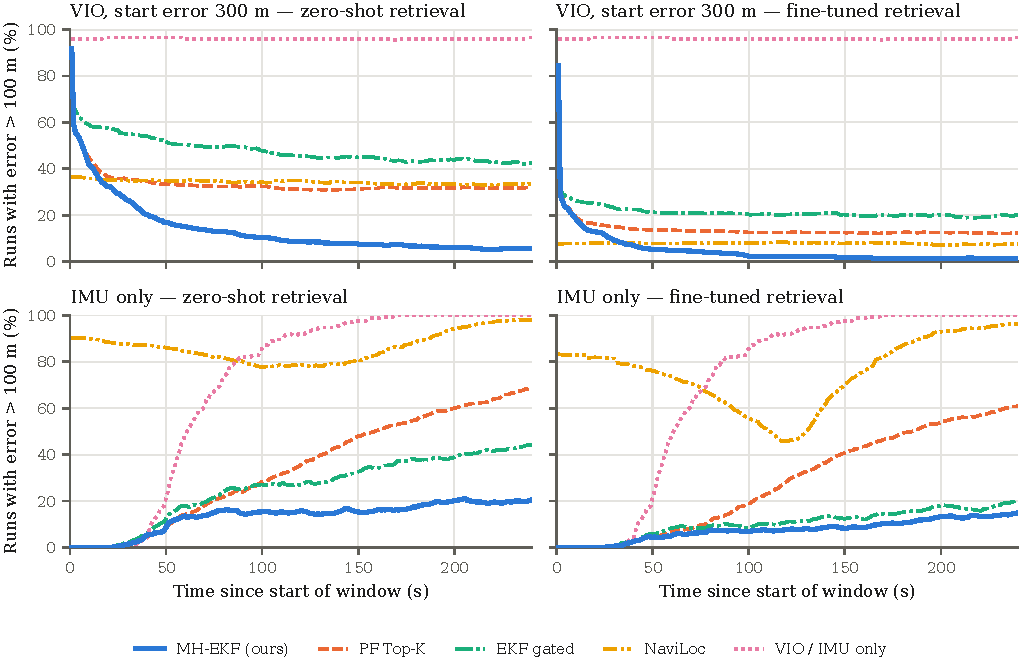
\includegraphics[width=0.92\textwidth]{figs/fig_lost_long.pdf}
  \caption{Fraction of runs with error above 100\,m as a function of time within the 240-s window, AerialVL
  \texttt{long\_trajtr} test flights. Top: wrong start ($\sigma=300$\,m) with VIO; bottom: IMU only. Left: zero-shot
  retrieval; right: fine-tuned retrieval.}
  \label{fig:lost}
\end{figure*}

\begin{figure}[t]
  \centering
  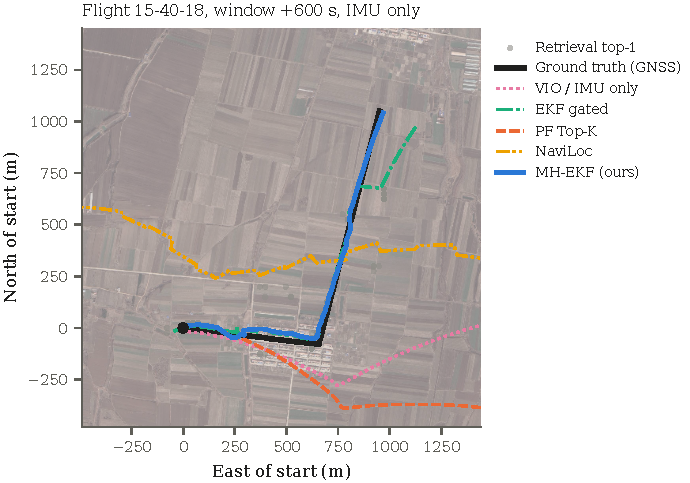
\includegraphics[width=\columnwidth]{figs/fig_traj_example.pdf}
  \caption{An IMU-only window of test flight 2023-03-18-15-40-18 (fine-tuned LPN). The window was \emph{selected} to
  illustrate a typical failure of the baselines (largest p95 gap between PF and MH-EKF among windows where MH-EKF
  stays below 100\,m); it is not a representative window.}
  \label{fig:traj}
\end{figure}

\subsection{Ablation}\label{sec:ablation}
\IfFileExists{tables/ablation.tex}{\begin{table*}[t]
\centering
\caption{Ablation of MH-EKF (one factor changed at a time; LPN head, 3 seeds; test data, analysis only --- the design was frozen on validation data before). p95 error in metres (\% runs lost). $^\blacktriangle$/$^\triangledown$: p95 at least 10\,\% worse/better than the full method. --: run not available.}
\label{tab:ablation}
\setlength{\tabcolsep}{3.5pt}
\small
\begin{tabular}{lcccccccc}
\toprule
 & \multicolumn{4}{c}{AerialVL long flights, fine-tuned retrieval} & \multicolumn{4}{c}{DenseUAV test campuses} \\
\cmidrule(lr){2-5}\cmidrule(lr){6-9}
Variant & VIO & IMU & VIO+$\epsilon_0$ & IMU+$\epsilon_0$ & VIO & IMU & VIO+$\epsilon_0$ & IMU+$\epsilon_0$ \\
\midrule
MH-EKF v3 (full) & 48 (2) & 180 (28) & 66 (4) & 388 (31) & 6 (0) & 11 (0) & 6 (0) & 11 (0) \\
\midrule
single hypothesis ($M=1$) & 49 (2) & 482$^\blacktriangle$ (29) & 752$^\blacktriangle$ (39) & 1493$^\blacktriangle$ (53) & 6 (0) & 12 (1) & 688$^\blacktriangle$ (17) & 800$^\blacktriangle$ (17) \\
$M=3$ & 48 (2) & 230$^\blacktriangle$ (28) & 214$^\blacktriangle$ (7) & 702$^\blacktriangle$ (32) & 6 (0) & 11 (0) & 6 (0) & 11 (0) \\
$M=5$ & 48 (2) & 209$^\blacktriangle$ (28) & 351$^\blacktriangle$ (9) & 764$^\blacktriangle$ (34) & 6 (0) & 11 (0) & 6 (0) & 11 (0) \\
$M=20$ & 48 (2) & 164 (28) & 61 (4) & 258$^\triangledown$ (30) & 6 (0) & 11 (0) & 6 (0) & 11 (0) \\
top-1 only ($K=1$) & 50 (3) & 246$^\blacktriangle$ (35) & 73 (6) & 356 (37) & 7 (0) & 12$^\blacktriangle$ (1) & 7 (0) & 13 (1) \\
$K=3$ & 48 (2) & 204$^\blacktriangle$ (30) & 116$^\blacktriangle$ (6) & 369 (33) & 6 (0) & 11 (1) & 7 (0) & 12 (0) \\
$K=5$ & 49 (2) & 182 (30) & 126$^\blacktriangle$ (6) & 412 (32) & 6 (0) & 11 (0) & 6 (0) & 11 (0) \\
gate $\chi^2_{0.95}$ & 48 (1) & 199$^\blacktriangle$ (30) & 61 (4) & 341$^\triangledown$ (32) & 6 (0) & 11 (1) & 6 (0) & 11 (1) \\
gate $\chi^2_{0.999}$ & 48 (2) & 103$^\triangledown$ (27) & 121$^\blacktriangle$ (5) & 612$^\blacktriangle$ (31) & 7 (0) & 12 (0) & 7 (0) & 12 (0) \\
no gate & 49 (3) & 119$^\triangledown$ (29) & 248$^\blacktriangle$ (6) & 919$^\blacktriangle$ (32) & 7 (0) & 12 (0) & 7 (0) & 12 (0) \\
no re-acquisition & 48 (2) & 186 (28) & 66 (4) & 395 (31) & 6 (0) & 11 (0) & 6 (0) & 11 (0) \\
re-acq.\ anywhere & 880$^\blacktriangle$ (28) & 1273$^\blacktriangle$ (41) & 1163$^\blacktriangle$ (28) & 1535$^\blacktriangle$ (42) & 6 (0) & 11 (0) & 6 (0) & 11 (0) \\
re-acq.\ $3\sigma+v_{\max}\Delta t$ & 53$^\blacktriangle$ (14) & 131$^\triangledown$ (32) & 167$^\blacktriangle$ (16) & 266$^\triangledown$ (35) & 6 (0) & 11 (0) & 6 (0) & 11 (0) \\
lost rule: best child & 48 (2) & 181 (28) & 66 (4) & 388 (31) & 6 (0) & 11 (0) & 6 (0) & 11 (0) \\
\bottomrule
\end{tabular}
\end{table*}
}{}
\Cref{tab:ablation} changes one component at a time (LPN head, test data; analysis only).
\emph{Multiple hypotheses} are the decisive component: with a single hypothesis the wrong-start scenarios collapse
(p95 above 680\,m on both datasets) while the known-start VIO case is unchanged.
\emph{Using the Top-$K$ candidates} instead of the top-1 mainly reduces the lost fraction with an IMU only.
\emph{Gating} is a trade-off: removing it degrades the wrong-start scenarios, but slightly improves the IMU-only p95 on
AerialVL, where an IMU-driven hypothesis is less often supported by an in-gate candidate.
\emph{Re-acquisition} as designed is almost never triggered: disabling it changes the results by a few metres at most,
whereas re-acquiring anywhere destroys the AerialVL results (p95 0.9--1.5\,km on the long flights with fine-tuned retrieval, and 0.7--2.8\,km across all AerialVL configurations), because long aliasing chains then
capture the filter. Allowing the re-acquisition radius to grow with time ($3\sigma+v_{\max}\Delta t$, $v_{\max}=10$\,m/s) is a trade-off: it lowers the IMU-only p95 on the long flights (180\,$\rightarrow$\,131\,m) but raises the lost fraction everywhere on AerialVL (e.g., 1.7\,$\rightarrow$\,14\,\% with VIO, 4.4\,$\rightarrow$\,16\,\% with a wrong start). The rule that decides when the track is lost (best child vs.\ no in-gate candidate) has no measurable effect, consistently with re-acquisition being rare; on DenseUAV none of the re-acquisition variants changes the result. The benefit of our rule is therefore that it prevents harmful jumps, not that it recovers lost tracks; a simpler filter without re-acquisition would perform the same on our data.
\emph{Bank size.} Fewer hypotheses ($M=3,5$) degrade the wrong-start and IMU-only scenarios on AerialVL, and $M=20$ is better than our $M=10$ in several hard cells (long flights, IMU with wrong start: 388\,$\rightarrow$\,258\,m) and never worse by more than 10\,\%; $M=10$, chosen on validation data, is therefore not saturated, and we keep it to respect the frozen design. \emph{Number of candidates and gate level} ($K\in\{3,5\}$, $\chi^2_{0.95}$, $\chi^2_{0.999}$) give mixed results without a uniformly better setting. On DenseUAV, where retrieval is strong, none of these factors matters except the single-hypothesis case.

\subsection{Runtime}
Per 1-Hz tick, on one CPU core in pure Python/NumPy, MH-EKF costs 0.47\,ms with VIO and 3.6\,ms with an IMU (100-Hz propagation of up to 10 EKFs), against 2.6\,ms and 24\,ms for the 2\,000-particle filter and 0.17\,ms and 1.6\,ms for the single EKF. The retrieval descriptor (ViT-S, image and its mirror) takes 13.8\,ms on an idle RTX~3050 laptop GPU and the Top-10 search over the 28\,340 tiles 2--4\,ms on one core, so the whole pipeline uses about 2.5\,\% of the 1-s budget. \todo{Optionally measure on an embedded board (e.g., Jetson).}

% =====================================================================================================
\section{Limitations}
\begin{itemize}
  \item \textbf{Simulated inertial data.} VIO and IMU are simulated from the ground-truth trajectories on both datasets.
  Real inertial logs of AerialVL exist as GeoVINS rosbags~\cite{li2025geovins} and are the next step. \todo{F-5: real IMU.}
  \item \textbf{One test day.} The eight AerialVL test flights were recorded on the same day over one area; bootstrap
  intervals over three or five flights are coarse.
  \item \textbf{Fine-tuned retrieval sees the test area.} It is trained on other days over the same map and does not
  show generalization to new areas; the zero-shot rows of \cref{tab:aerialvl} are the conservative result.
  \item \textbf{Re-implemented competitor.} NaviLoc has no public code; our version follows the published algorithm,
  without its heading-rectification stage. FoundLoc, GeoVINS and SWA-PF are not compared. \todo{Decide whether to add one.}
  \item \textbf{IMU-only flights remain unsolved}: about a third of the long-flight windows are lost.
\end{itemize}

\section{Conclusion}
Treating cross-view retrieval as a multimodal, outlier-contaminated measurement and tracking a small bank of hypotheses
bounds the tail errors that make single-frame retrieval unusable for navigation. On real flights the gain over simpler
filters is small when VIO is good and the start is known, and large when the start is wrong, the motion source is an
IMU, or retrieval is weak. Real inertial data and a broader set of competitors are the main open points.

\bibliographystyle{IEEEtran}
\bibliography{refs}

\end{document}
